\documentclass[sigconf]{acmart}

\AtBeginDocument{%
  \providecommand\BibTeX{{%
    \normalfont B\kern-0.5em{\scshape i\kern-0.25em b}\kern-0.8em\TeX}}}

\copyrightyear{2020} 
\acmYear{2020} 
\setcopyright{rightsretained} 
\acmConference[VINCI 2020]{The 13th International Symposium on Visual Information Communication and Interaction}{December 8--10, 2020}{Eindhoven, Netherlands}
\acmBooktitle{The 13th International Symposium on Visual Information Communication and Interaction (VINCI 2020), December 8--10, 2020, Eindhoven, Netherlands}\acmDOI{10.1145/3430036.3432753}
\acmISBN{978-1-4503-8750-7/20/12}

\usepackage{subfig}
\usepackage{csquotes}
\usepackage[binary-units=true]{siunitx}
\usepackage{tikz}
\usetikzlibrary{calc,positioning,spy}

\begin{document}

\title{Depicting Uncertainty in 2.5D Treemaps}

\author{Daniel Limberger}
\email{daniel.limberger@hpi.de}
\affiliation{%
  \institution{Hasso Plattner Institute,\\Faculty of Digital Engineering,\\University of Potsdam, Germany}
}
\author{Matthias Trapp}
\email{matthias.trapp@hpi.de}
\affiliation{%
  \institution{Hasso Plattner Institute,\\Faculty of Digital Engineering,\\University of Potsdam, Germany}
}
\author{J{\"u}rgen D{\"o}llner}
\email{juergen.doellner@hpi.de}
\affiliation{%
  \institution{Hasso Plattner Institute,\\Faculty of Digital Engineering,\\University of Potsdam, Germany}
}

\renewcommand{\shortauthors}{D. Limbeger, M. Trapp, and J. D{\"o}llner}

\begin{abstract}
  A truthful and unbiased display of data using information visualization requires detecting and communicating uncertainty.
  Uncertainty is often inherent in data or is introduced by data processing and visualization (e.g., visual display of accumulated data) but frequently not accounted for.
  This paper discusses the suitability of advanced visual variables such as sketchiness, noise, nesting-level contouring, and color weaving for communicating uncertainty.
\end{abstract}

\begin{teaserfigure}
  \centering
  \begin{tikzpicture}[spy using outlines={white, rectangle, magnification=2.0, size=52, connect spies, every spy on node/.append style={thin}},inner sep=0pt, outer sep=0pt]
    % LEFT MOST
    \node[anchor=west](weaving0) at (-0.5\linewidth,0) {%
        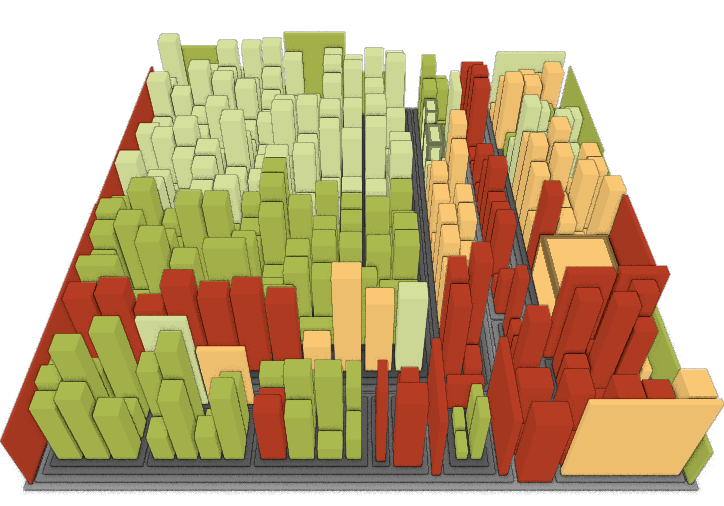
\includegraphics[trim=0 0 80 10, clip, width=0.24\textwidth]{./resources/color-weaving-4.png}};%
    \spy on ($(weaving0)+(1.1, -0.6)$) in node at ($(-1.0, 1.05)+(weaving0.center)$);
    % LEFT
    \node[anchor=west, inner sep=0pt, outer sep=0pt](weaving1) at (-0.25\linewidth,0) {%
        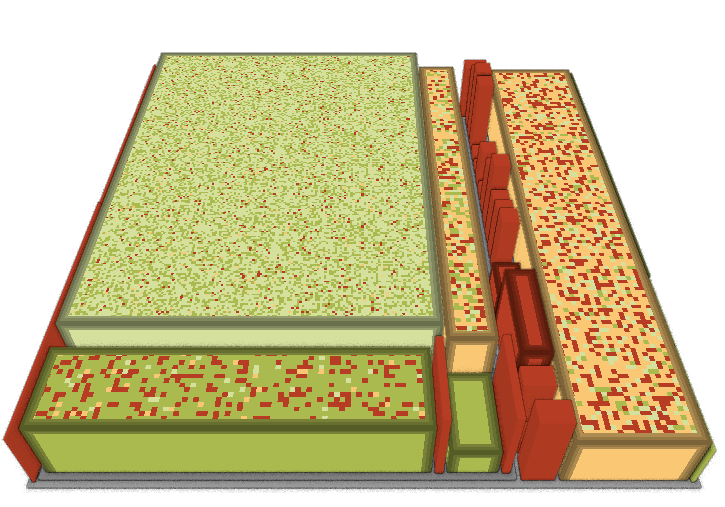
\includegraphics[trim=0 0 80 10, clip, width=0.24\textwidth]{./resources/color-weaving-3.png}};%
    \spy on ($(weaving1)+(1.1, -0.6)$) in node at ($(-1.0, 1.05)+(weaving1.center)$);
    % RIGHT
    \node[anchor=east, inner sep=0pt, outer sep=0pt](noise0) at (0.25\linewidth, 0) {%
        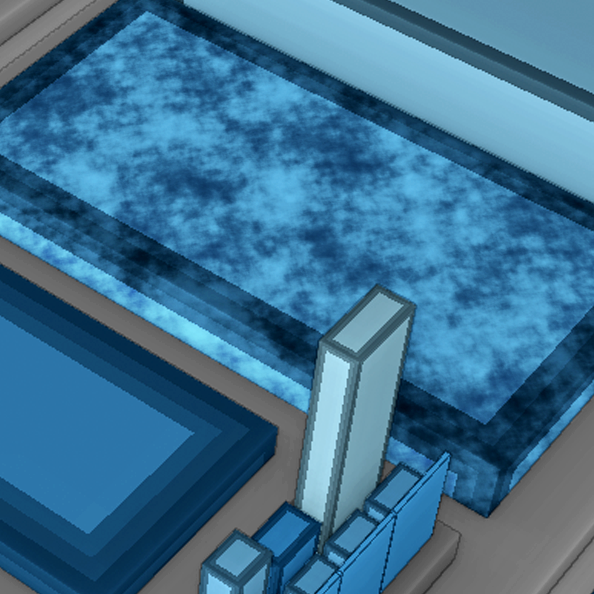
\includegraphics[trim=00 00 00 160, clip, width=0.24\textwidth]{./resources/aggregation-noise-distribution-a-cropped.png}};%
    \spy on ($(noise0.center)+(1.3, -0.6)$) in node at ($(-1.0, 1.05)+(noise0.center)$);
    % RIGHT MOST
    \node[anchor=east, inner sep=0pt, outer sep=0pt](noise1) at (0.5\linewidth, 0) {%
        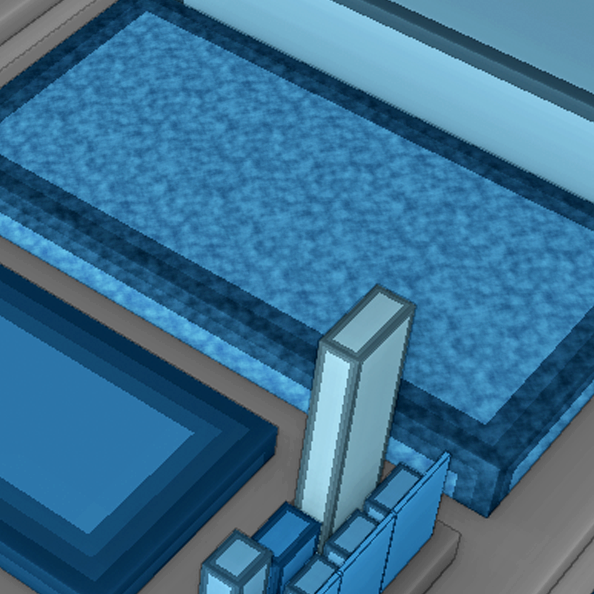
\includegraphics[trim=00 00 00 160, clip, width=0.24\textwidth]{./resources/aggregation-noise-distribution-b-cropped.png}};%
    \spy on ($(noise1.center)+(1.3, -0.6)$) in node at ($(-1.0, 1.05)+(noise1.center)$);
  \end{tikzpicture}
  \vspace{-0.6cm}
  \caption{Left: a software map depicting development activity on code units, without and with color weaving and nesting-level contouring applied for the rendering of aggregates. Right: utilization of Perlin noise of low and high frequencies depending on the underlying data distribution. The nesting-level contouring denotes the maximum depth of the collapsed data sub-tree.}
  \label{CW:Fig:Teaser}
\end{teaserfigure}

\maketitle

\section{\uppercase{Introduction}}
\label{CW:Sec:Introduction}

\noindent
The expressiveness of any visualization is subject to and limited by the visual variables used to encode data (attributes).
With careful consideration, multiple visual variables can be superimposed to one another, without significantly reducing their effectiveness.
We use recently introduced visual variables~\cite{limberger2019-advanced} and discuss their potential for the representation of uncertainty in 2.5D treemaps. %
A truthful and unbiased depiction of the underlying data is relevant, especially when visual analytics tools become regularly used communication artifacts. %
Haber and McNabb differentiate between visualization of uncertainty and uncertainty of visualization~\cite{Haber1990}. 
The first covers uncertainties that inherent to the quality of data, correctness of measurements, trustworthiness of assumptions, as well as probability of trend forecasts.
The latter is inherent to accumulated or sampled data, e.g., when using level-of-detail techniques.
A visual aggregate is a specialized node representation that can be used to resolve clutter, reduce the cognitive load, or emphasize regions-of-interest, as recently shown for \emph{software maps}~\cite{limberger2017-aggregation}. %
We differentiate between the (1) \emph{attribute uncertainty} and (2) \emph{distribution uncertainty}.
The first can be associated directly to mapped attributes and is depicted using the additional visual variables on leaf nodes.
For the latter, the same techniques can be applied on aggregates, 
which, however, introduces information loss and increases uncertainty by means of (1) obfuscating whether or not to explore and investigate further and (2) hindering identification of relevant nodes and outliers.
\emph{Color weaving}~\cite{Hagh-Shenas2007}, \emph{sketchiness}~\cite{Boukhelifa2012,limberger2016-sketchy}, \emph{nesting-level contouring}~\cite{limberger2017-aggregation}, \emph{perlin noise}~\cite{Djurcilov2002,Coninx2011}, and \emph{chart-based rendering and labeling} can be used to mitigate these issues.

\section{Attribute Uncertainty}

In order to allow for additional depiction of uncertainty, %
we use sketchiness \cite{Boukhelifa2012,limberger2016-sketchy} or Perlin noise \cite{Djurcilov2002,Coninx2011} in addition to node size, color, and height.
Both approaches can depict data with inherent quality information or uncertainty data available, such as sampling rate, currentness, error rate, and relevance.
Sketchiness, however, seems to be better suited to convey multiple distinguishable degrees of uncertainty. %
When applied to aggregates, %
we superimposed nesting-level contours for both techniques.
Height and color mapping can still be used, e.g., for encoding the existence of outliers using aggregation operators~\cite{limberger2017-aggregation}. %

Sketchiness can be configured in terms of style (pattern, outline, stroke thickness) and intensity.
Increased uncertainty is mapped to increased sketchiness intensity using a 5-point Likert scale (none, minor, moderate, high, and severe/major). %
Specifics of that mapping depend on the actual task and we assume uncertainty to play a secondary role during analysis. 
If uncertainty is the primary concern of a task, it should be mapped directly to color or height instead.

When using Perlin Noise, the depth or level of aggregated nodes can be mapped to noise frequency. 
This is also useful when different levels of a treemap have different semantics, e.g., code units within a file system, budgets, or team composition.
The amplitude of the noise is used to encode the degree of uncertainty and can be mapped directly as well as continuously. 

\section{Distribution Uncertainty} 

For the visual encoding of data distribution three techniques can be taken into account: (1) Perlin Noise with  weighted octaves, (2) color weaving, and (3) chart glyphs~\cite{soares2018-adaptiveglyphs}. 
The use of Perlin Noise~(Figure~\ref{CW:Sec:Introduction}) takes advantage of combining multiple octaves with varying degrees of intensity, thereby resulting in low or high frequent components that can be used to indicate data distribution as well as existence of outliers.
Alternatively, chart-depicting glyph accurately encode distribution in a well known manner, e.g., pie charts or box plots (Figure~\ref{CW:Fig:Glyphs}).
Especially for small aggregates, tiny glyphs can be placed on top of aggregates, e.g., next to their labels.

\begin{figure}[b]
  \begin{tikzpicture}[inner sep=0pt, outer sep=0pt]%
    \node[](glyph0){%
      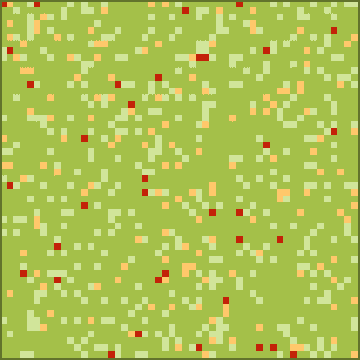
\includegraphics[width=0.24\linewidth]{./resources/MC-CW-normal1.png}};%
    \node[right=0.5mm of glyph0.east, inner sep=0pt, outer sep=0pt](glyph1) {%
      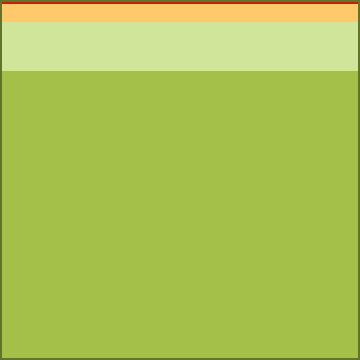
\includegraphics[width=0.24\linewidth]{./resources/MC-SB-normal1.png}};%
    \node[right=0.5mm of glyph1.east, inner sep=0pt, outer sep=0pt](glyph2) {%
      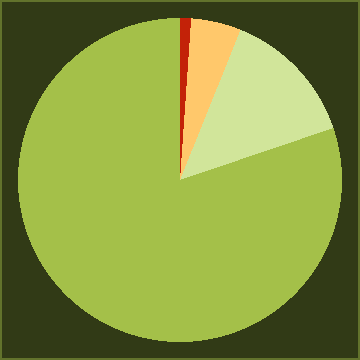
\includegraphics[width=0.24\linewidth]{./resources/MC-P-normal1.png}};%
    \node[right=0.5mm of glyph2.east, inner sep=0pt, outer sep=0pt](glyph3) {%
      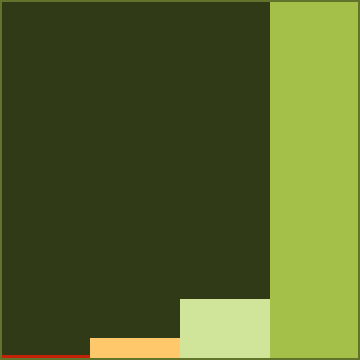
\includegraphics[width=0.24\linewidth]{./resources/MC-B-normal1.png}};%
  \end{tikzpicture}
  \caption{Distribution representations to color weaving (left) using glyphs charts, rendered onto the top faces of aggregates: stacked chart, pie chart, and bar chart.}
  \label{CW:Fig:Glyphs}
\end{figure} 

The uncertainty display of aggregates needs to adhere to \emph{visual summary} (convey information about underlying data), \emph{discriminability} (distinguishable presentation of aggregates and data items), and \emph{interpretability} (remain correctly interpretable within the visual mapping)~\cite{elmqvist2010-aggregation}.
Since color weaving \cite{Hagh-Shenas2007} is based on color mixing with a given color map, it especially supports interpretability and further improves \emph{fidelity} (aggregates may lie about their underlying data).
It can mitigate the uncertainty of the visualization by explicitly depicting it.
This in turn allows to guide the user during interactive exploration, e.g., whether or not to investigate certain nodes, identify relevant nodes, detect outlier, or prevent data to be accumulated in misleading ways.
Color weaving can also reflect the underlying data with respect to other attributes, resulting in unweighted and weighted depictions (Figure~\ref{CW:Fig:Weighting}). 

\begin{figure}[t]
  \begin{tikzpicture}[inner sep=0pt, outer sep=0pt]%
    \node[](aggregated0){%
      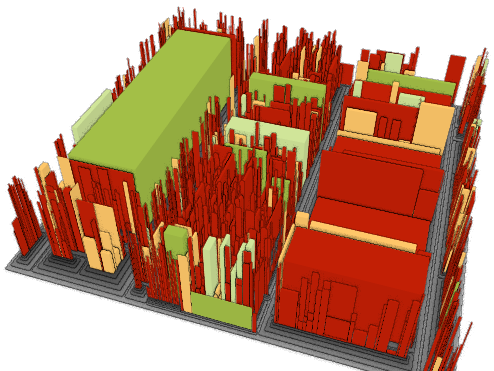
\includegraphics[trim=20 80 80 20,clip,width=0.33\linewidth]{./resources/teaser-normal-2.png}};%
    \node[right=0.5mm of aggregated0.east, inner sep=0pt, outer sep=0pt](aggregated1) {%
      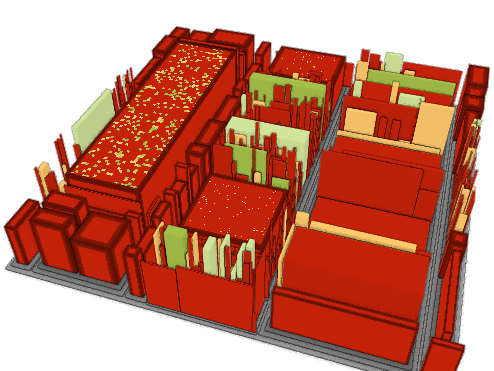
\includegraphics[trim=20 80 80 20,clip,width=0.33\linewidth]{./resources/teaser-unweighted-2.png}};%
    \node[right=0.5mm of aggregated1.east, inner sep=0pt, outer sep=0pt](aggregated2) {%
      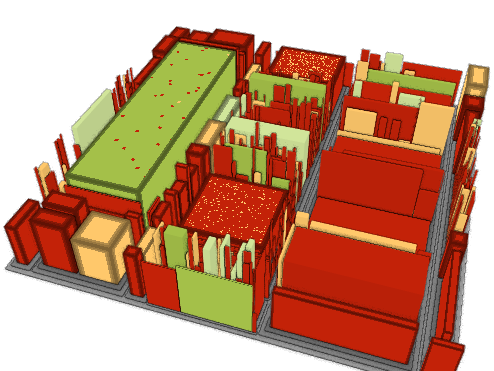
\includegraphics[trim=20 80 80 20,clip,width=0.33\linewidth]{./resources/teaser-weighted-2.png}};%
  \end{tikzpicture}
  \caption{2.5D Treemap using, unweighted (middle) and weighted (right) color weaving for the visual display of uncertainty of accumulated software system data.}
  \label{CW:Fig:Weighting}
\end{figure}

The patch size specifies the resolution for any mapping. 
For distribution mapping, for example, a bigger patch size (e.g., $16 \times 16$) allows for a more accurate distribution depiction.
Furthermore, we adjust the mapping to always account for single occurrences within a value range in order to not lie about the underlying data (note that this marginally distorts the distribution display).
Another important parameter is the overall grid scale.
For large treemaps with deep nesting levels, the grid scale should be adjusted per hierarchy level.
Our implementation also allows for weighted data distribution display (Figure~\ref{CW:Fig:Weighting}) intended for tasks where qualitative color scales with more color classes are used. 
This way, we can emphasize specific classes explicitly.

\section{\uppercase{Discussion \& Future Work}}
\label{CW:Sec:ResultsAndDiscussion}

\noindent %
We found that both Perlin noise and color weaving can be combined with nesting-level contours without limitations.
Furthermore, the discriminability of aggregates can be increased and preexisting shading, contouring, shadowing, or highlighting remains unaffected.
There are edge cases, however, that require additional adjustment w.r.t. the number of noise octaves, patch size, or the glyph charts placement and scale.
In terms of visual software analytics, we explored different data mappings for data item uncertainty, e.g., developer participation, developer activity, as well as data distribution uncertainty for common software metrics and their evolution.
Future work could investigate whether color weaving (1) accurately conveys distribution data and (2) outperforms well-known plotting approaches or single-color aggregation strategies.
The results would enable automated selection of the best-fit visualization for a given uncertainty and screen estate.

\bibliographystyle{ACM-Reference-Format}
\bibliography{uncertainty}

\end{document}
\endinput
